\chapter{Introduction}
\label{introduction}
\index{Introduction@\emph{Introduction}}%


In recent years wireless LAN technology has become ubiquitous. Wi-Fi access points have become virtually trivial to install, and nearly everyone carries a Wi-Fi capable mobile device in their pocket. It is also the case that much research has been done on various methods of location estimation. It follows, then, that location estimation that leverages Wi-Fi would be a valuable topic, and in fact much research has already been done in the space, including \cite{ito2005bayesian}, \cite{liu2007survey}, \cite{kawaguchi2009wifi}, \cite{hotta2012robust}, and \cite{nagaosa2012dept}. 

The benefits of using Wi-Fi for location estimation are manifold. For instance, while the Global Positioning System is in many ways the premier method for location estimation in the world \cite{bajaj2002gps}, GPS signals are often unreliable indoors \cite{xiong2012towards}, making it a poor choice for any indoor location estimation. Location systems that use other mechanisms such as RFID \cite{toplan2012rfid}, ultrasound \cite{priyantha2005cricket}, or geomagnetism \cite{chung2011indoor} are difficult to setup, require specialized hardware, and ultimately can only be used for a single purpose. Wi-Fi based location estimation solves all of these problems. Wi-Fi signals are readily available indoors. Wi-Fi is relatively cheap and easy to setup, and in many cases existing access points can be leveraged.

\section{Definitions}
\index{Definitions@\emph{Definitions}}%

There are a few terms that will be used throughout this paper that it is important to define early. Understanding these definitions will help make clear the purpose of this paper and its contributions. 

\paragraph{Signal Strength vs. RSSI}

Much of the research involving location estimation with Wi-Fi signal strength refers to the measured power present in the radio signal as the Received Signal Strength Indicator (RSSI). While in general terms this moniker is good enough, in truth, the IEEE 802.11 specifications \cite{ieee802.11} do not indicate a specific relationship between RSSI and the actual power level as measured in either milliwatts (mW) or Decibel-milliwatts (dBm). As such, manufactures are free to provide their own arbitrary units, and RSSI measurements are generally found to be integer values greater than 0. Because of this inconsistency, Honeycomb does not use RSSI, favoring instead what we refer to as simply "signal strength". For our purposes, signal strength is a measure of the power present in the Wi-Fi signal as measured in dBm. dBm is a measurement relative to 1 mW of power, where 0 dBm is equal to 1 mW. Because dBm measurements are made on a logarithmic scale, we find our measurements to be negative integers between 0 and -100, where the measured value is the exponent in the logarithm. So, where 0 dBm is equal to 1 mW, -10 dBm is equal to .1 mW, -20 dBm is equal to .01 mW, and so on. Measuring signal strength in this way allows Honeycomb to maintain consistent tracking across signal strength measurement platforms, and thus makes Honeycomb a more diverse and viable product.


\paragraph{Fingerprint}
Throughout this paper will we refer to fingerprints. In this context, a fingerprint is a set of Wi-Fi signal strength measurements taken from a set of Wi-Fi access points at a specific point in a given space. 

\begin{figure}[htb] % Imported eps example.
	\begin{center}
		\ 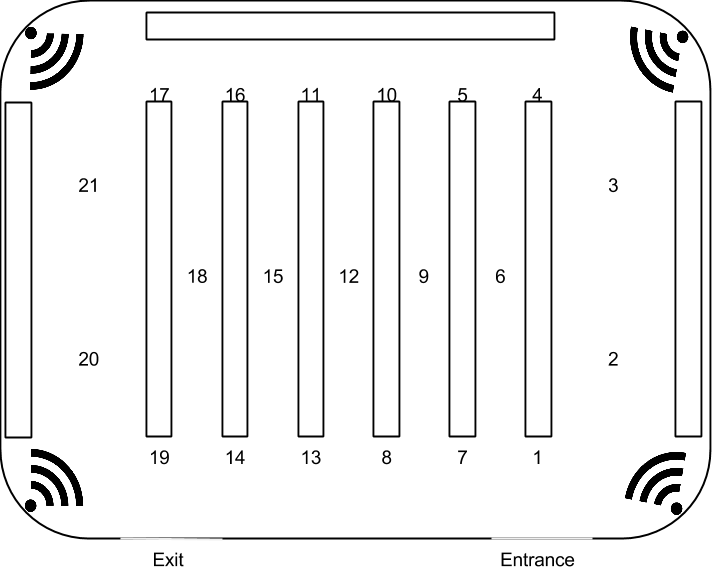
\includegraphics[width=4in,height=3in]{ExampleLocation.png}
		\caption{An example of a location with labeled measurement points}
		\label{storeexample}
	\end{center}
\end{figure}


\paragraph{Fingerprint Session}

While the concept of the Wi-Fi fingerprint is relatively common, here we introduce a new concept that will enable a Honeycomb installation to maintain its value over time: the fingerprint session. A fingerprint session is the complete set of fingerprints from all measurement points in a space at measurement time. Because the internal layout of any given space can change over time, causing issues with blocking and reflection of Wi-Fi signals, Honeycomb has built in the ability to re-fingerprint the entire location at any time so that the measurements can be as precise as possible. Figure \ref{storeexample} shows an example location with aisles like that of a grocery store. It includes four Wi-Fi access points and numbered labels for points that may be considered relevant for location estimation. A single fingerprint session in this space would be the complete set of Wi-Fi signal strength measurements from all four access points at every numbered location. 


\paragraph{User Track}
A user track differs from a fingerprint in that it represents a single user's movement through the space. Thus, a user track is composed of a set of timestamps, each of which is associated with a set of signal strength measurements for each of the access points in the space. Figure \ref{usertrackexample} shows an example of a user track. In this example, the small dots represent the user's actual path through the space, while each large dot represents a timestamped set of signal strength measurements. Thus it can be seen that in this example the user walked at a relatively constant pace through the space, slowing down four times near locations 5, 7, 14, and 17. For location estimation purposes, Honeycomb will compare a given user track to the most recent fingerprint session for the given space. 


\begin{figure}[htb] % Imported eps example.
	\begin{center}
		\ 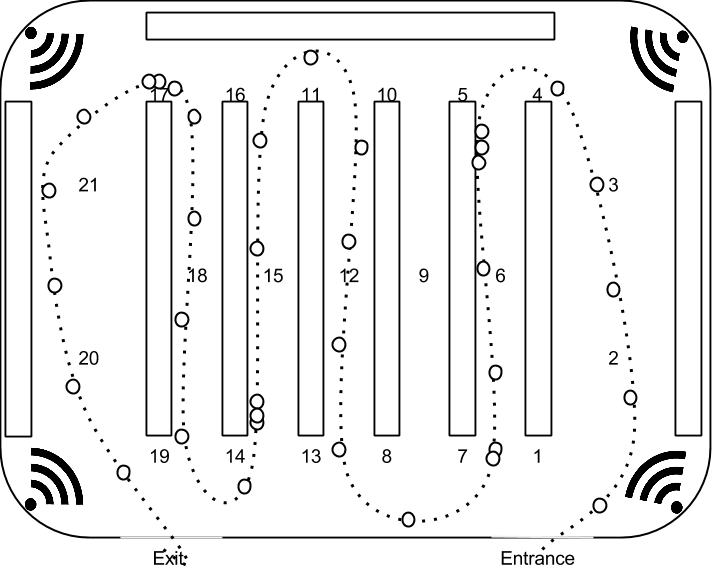
\includegraphics[width=4in,height=3in]{ExampleUserTrack.png}
		\caption{An example user track}
		\label{usertrackexample}
	\end{center}
\end{figure}


\section{Motivation}
\index{Motivation@\emph{Motivation}}%

Wi-Fi based location estimation is a well researched topic \cite{liu2007survey}. The goal of Honeycomb is to leverage that research and build an indoor location tracking system which is suitable for deployment in a real world scenario.  As such, Honeycomb includes an Android application capable of fingerprinting a space, and an API which is deployed to the web for uploading both fingerprints and user track data. The web application also executes the location estimation algorithm, and provides a user interface for browsing the user track data. Honeycomb itself remains agnostic of the mechanism used to gather the user's Wi-Fi signal strength data. By decoupling Honeycomb in this way, we allow Honeycomb to be used in multiple scenarios in which a specialized user track gathering mechanism is desired. 

User privacy is also a major motivating factor in our work. By only performing location estimation based on signal strength and timestamp data passively gathered on the Wi-Fi capable device, we have avoided the pitfalls of systems that require the mobile device to send out a beacon \cite{ito2005bayesian} \cite{xiong2012towards} which can be intercepted by malicious third parties. Additionally, the offline nature of the location estimation algorithm greatly simplifies the entire process, as real time location estimation is still a highly volatile field \cite{turner2011empirical}. It also helps provide an additional layer of privacy protection for the user, as the data can easily be decoupled from any identifying information before processing. There are, of course, motivations for real time trackers as well, which Honeycomb does not address.
 
 
\section{Contribution}
\index{Contribution@\emph{Contribution}}%

While there has been much research done in the space (see chapter \ref{related}), to the author's knowledge, there does not yet exist a product on the market that achieves true location estimation via Wi-Fi signal strength measurements. Honeycomb is such a product. Honeycomb provides tools on the web for site administrators to manage their locations and view individual user tracks. It also includes an API through which fingerprints and user tracks can be uploaded, and an Android application capable of doing the fingerprinting and uploading the results to Honeycomb through the API. 


\section{User Stories}
\index{User Stories@\emph{User Stories}}%

We envision Honeycomb being deployed in multiple different scenarios. Essentially, wherever there is a desire to track a person's movements through a bounded space, we believe Honeycomb to be part of a viable solution. In this section, we describe two such scenarios.

\subsection{The Grocery Store}
The canonical example, and the one to which we will refer throughout this paper, is the retail establishment that wishes to track customer movements through their space. In this case, we use the example of the grocery store. The grocery store lends itself well to this scenario due to the fact that stores are generally rather large in size and that there is a general expectation that its customers will spend most of their time moving around the space. In this scenario, we see two major benefits of customer location tracking.  Although we've chosen the grocery store for this scenario, these same benefits could be applied to similar scenarios, such as large conferences with multiple rooms and displays. In this scenario, we see two major benefits to the grocery store: 

\paragraph{Visibility}

High visibility of products is a valuable commodity in any retail environment. Each store can use aggregate data about its customers' movements through the space to identify key, high traffic areas, and sell shelf space or ad space accordingly. Additionally, \cite{shukla2013effects} shows that customers respond to engaging store layouts, which can be facilitated by customer movement data. Similarly, a conference can identify high traffic areas and place sponsor ads, or other information valuable to attendees, at the site.

\paragraph{Flow Control}

Data about how people move through a space can be used to identify bottlenecks or other poorly designed traffic areas and improve them in order to provide a better user experience for patrons. In the context of a grocery store, this could result in a generally happier clientele, which means more repeat business \cite{shukla2013effects}. At a conference, this data could be used to identify popular booths, and rearrange them in such a way that will cause traffic to flow in desired patterns, either to eliminate bottlenecks or to direct traffic flow past more sponsors.

\subsection{Security Guards}

For security companies, a critical component of their service is often regular patrolling of the space by a human being. For this reason, it is crucial for the security company to make absolutely sure that the security guard actually goes on their patrols. This is often accomplished via RFID stations or QR codes located throughout the space that the guard must scan in order to prove that they were there. However, this scanning requires the security guard to be both mentally and visually distracted for the length of time required to make the scan, and therefore creates a weak point in their security that can be exploited. Passive tracking of the security guard via Wi-Fi signal strength polling eliminates this distraction, while still maintaining the necessary tracking. 

Note that in the above examples, the method by which the polling data is transferred from the individual's Wi-Fi capable device into Honeycomb may be dramatically different. In the case of the grocery store, there may be some desire on the part of store management to evaluate the data before transferring it to Honeycomb, for example to credit the customer's account for their incorporated rewards system, which may be necessary as a motivation for the user to allow themselves to be tracked. A grocery store's general patterns of ingress and egress provide a natural place for the data to be collected, possibly over Wi-Fi itself, so as to be as unobtrusive to the customer as possible. Conversely, in the example of the security guard, there may not be a convenient area in which to place a data collector, since you may be tracking multiple security guards through multiple spaces, and it is not worth setting up a data collector for one individual in a given space. Additionally, obtrusiveness is not an issue, since reporting their position data is part of the security guard's  job. It is for this reason that Honeycomb remains agnostic of the user data gathering mechanism, in order to provide benefit in a wider variety of areas.


\section{Structure Of This Report}
\index{Structure Of This Report@\emph{Structure Of This Report}}%

The goal of this report is to provide context for the value of a Wi-Fi signal strength based indoor location tracking system and to describe the particular implementation of Honeycomb. In Chapter \ref{related} we discuss the state of Wi-Fi based location tracking and explain why we feel that the methods we chose were the best choices for Honeycomb.  In Chapter \ref{bumblebee} we present BumbleBee. Because Honeycomb remains agnostic of user track gathering mechanisms, we needed to choose a product that is capable of gathering user track data. BumbleBee is an independent, previously unpublished Wi-Fi signal strength measurement tool used to collect user tracks, and was co-written by the author of this paper. In Chapter \ref{tech-overview} we discuss the architecture of Honeycomb and the technologies on which it was built. In Chapter \ref{results} we present the testing procedures that were implemented and their results. In Chapter \ref{discussion} we discuss the results of our tests and the future of Honeycomb as a product.